\documentclass[11pt,a4paper]{article}
\usepackage{fouriernc}
\usepackage[latin1]{inputenc}
%\usepackage[T1]{fontenc}
\usepackage{paralist}
\newenvironment{enumin}%
% {\begin{inparaenum}[\hspace{1em}(1)]\hspace{-1em}\ignorespaces}%
   {\begin{inparaenum}[\hspace{0.6em}(1)]}%
   {\end{inparaenum}}
\usepackage{enumitem}
\usepackage{amsmath, amsfonts, amsbsy, bm}
\usepackage{graphicx}
\usepackage{color}
\usepackage{xspace}
\usepackage{booktabs}
\usepackage{siunitx}
\usepackage[colorlinks=true,linkcolor=black,urlcolor=black,hyperfootnotes=false]{hyperref}
%%%
\title{Dynamics of Structures 2010-2011\\\large 1st home assignment
  due on Tuesday 2011-06-17}
\date{}
\def\linka{http://en.allexperts.com/q/Microsoft-Word-1058/2009/8/embedding-pdf-file.htm}
\setcounter{tocdepth}{1}
\graphicspath{{xfig/}}
%%%
\begin{document}
\maketitle{}
\tableofcontents{}
\section*{Instructions}

For each of the \emph{six problems}, copy the text of the problem,
\emph{briefly} summarize the procedure you'll be using, detail all
relevant steps including part of intermediate numerical results as you
see fit, \emph{clearly state} the required answers. Scores
are${}\approx{}10, 20, 15, 15, 15, 25$.

Submit your homework by email before 14:30 or, if you prefer, hand in
your homework directly to me before the class.
\begin{itemize}
\item Handed in submissions must be printed or \emph{nicely}
  handwritten.
\item Email submissions \emph{must include} a PDF\footnote{a PDF as
    produced by Office or LaTeX or similar...no scans nor photos.}
  \footnote{Please check that all needed fonts are included in the
    file before sending. In doubt, \href\linka\linka.}  attachment
  with your solutions.  You can attach everything else is relevant for
  you (spreadsheets, your programs' sources) except Word files as I
  always encounter strange compability problems.
\end{itemize}
% +++++++++++++++++++++++++++++++++++++++++++
\section{Impact}
\[\input{xfig/impact.pdf_t}\]
\noindent A body of mass $m_1=\SI{120}{\kilogram}$ hits an undamped
\emph{SDOF} system, of unknown characteristics $k$ and $m_2$, with
velocity $\dot{x}_1=\SI{50}{\meter\per\second}$.

The collision is anelastic, i.e., the two masses are \emph{glued} together
and a measurement of the ensuing free oscillations gives the following
results:
\[ x_\text{max} =\SI{30}{\milli\meter},\qquad
   \dot{x}_\text{max}=\SI{60}{\milli\meter\per\second}.\]
%
Compute:
\begin{enumerate}
\item the total mass $m=m_1+m_2$
\item the mass $m_2$ of the impacted body,
\item the circular frequency of the insuing motion,
\item the spring stiffness $k$.
\end{enumerate}
%\clearpage
\section{Vibration Isolation --- Numerical Integration} 
A rotating machine, its mass $M=\SI{35000}{\kg}$, is rigidly connected
to the floor.

Due to unbalances, during steady-state regime the machine is subjected
to a harmonic force $p(t)=\SI{1}{\kilo\newton}\,\sin(2\pi\,\SI{5}\hertz\, t)$.

\subsection{Vibration Isolation}
Considering the floor fixed, design an appropriate suspension system
such that the steady-state transmitted force is reduced to
\SI{300}{\newton}.
\subsection{Numerical Integration}
When the machine is turned on, its full velocity is reached in
\SI{6}{\second}.  The angular velocity and the unbalanced load vary
linearly, from $0$ to their respective maximum values, i.e.,
\[p(t)=
\begin{cases}
  \SI{1}{\kilo\newton}\,\frac{t}{\SI{6}\second}\;
  \sin\left(2\pi\,\SI{2.5}{\hertz}\,\frac{t^2}{\SI{6}{\second}}\right) &  \SI{0}\second \le t \le \SI{6}\second,\\
  \SI{1}{\kilo\newton}\;\sin(2\pi\,\SI{5}{\hertz}\, t) &  \SI{6}\second\le t.
\end{cases}
\]
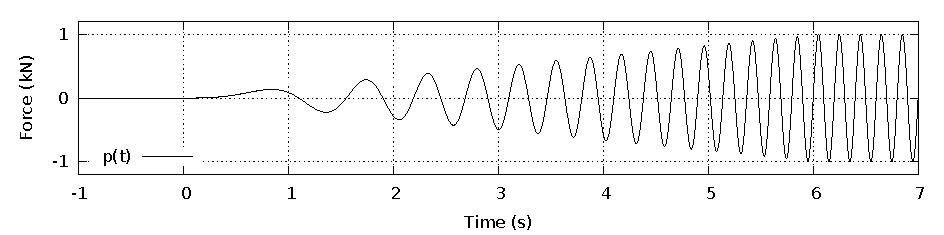
\includegraphics{p_of_t}

\bigskip\noindent Using the stiffness computed in the previous step,
find  the maximum absolute value of the displacement using either
the constant or the linear acceleration method and plot the response
in the interval $\SI{0}\second \le t \le \SI{10}\second$.
% +++++++++++++++++++++++++++++++++++++++++++
%
\section{Estimation of damping ratio}
You want to determine the mass $m$, the stiffness $k$ and the damping
ratio $\zeta$ of a one storey building that can be modeled as a single
degree of freedom system.

A series of 4 dynamical test is performed, loading the building with a
vibrodyne and measuring the amplitude $\rho$ and the phase difference
$\theta$ of the steady state motion (note that the measures of $\rho$
and $\theta$ are affected by a random measurement error).

In each test the load amplitude is $p_0=\SI{600}{\newton}$, while
the excitation frequencies $\omega_n$ (with $n=1,\ldots,4$) are
different.

The relevant data is summarized in the following table
\begin{center}
  \begin{tabular}{rcrr}
    \toprule 
    $n$ & 
    $\omega_n (\si{\rad\per\second})$ & 
    $\rho_n (\si{\micro\metre})$  &
    $\theta_n (\si{\deg})$\\
    \midrule
    1 & 40 & 12.39062 &   7.58258 \\
    2 & 50 & 41.09556 &  33.33505 \\
    3 & 60 & 18.07490 & 163.21210 \\
    4 & 70 &  7.11246 & 171.69968 \\
    \bottomrule
  \end{tabular}
\end{center}
Give your best estimate of $m$, $\zeta$ and $k$.
% +++++++++++++++++++++++++++++++++++++++++++
\section{Generalised Coordinates (rigid bodies)}

\[\input{xfig/newtrab.pdf_t}\]

\noindent The articulated system in figure, composed by
\begin{itemize}
\item two rigid bars, \begin{enumin}\item \textsf{ABC} and
  \item\textsf{CDE},
  \end{enumin}
\item three fixed constraints,
  \begin{enumin}
  \item a horizontal roller in \textsf{A},
  \item an internal hinge in \textsf{C} and
  \item a hinge in \textsf{E},
  \end{enumin}
\item two deformable constraints,
  \begin{enumin}
  \item a horizontal spring in \textsf{A}, its stiffness${}=k$ and
  \item a vertical dashpot in \textsf{C}, its damping
    coefficient${}=c$,
  \end{enumin}
\end{itemize}
is excited by a horizontal harmonic  force applied in \textsf{B},
\(p(t)=p_0\,\sin\omega t.\)

The vertical parts of the two bars, \textsf{AB} and \textsf{ED}, are
massless while both the horizontal parts, \textsf{BC} and \textsf{CD},
have a constant unit mass $\overline m$, with $\overline m\,L=m$.

\medskip\noindent Using $u_\textsf{A}$ (the horizontal displacement of
\textsf{A}) as the generalised coordinate
\begin{enumerate}
\item compute the generalised parameters $m^*$,  $c^*$ and $k^*$,
\item compute the generalised loading $p^*(t)$ and
\item write the equation of dynamic equilibrium.
\end{enumerate}
% +++++++++++++++++++++++++++++++++++++++++++
\section{Rayleigh quotient}
\label{sec:rayleigh}
\[\input{xfig/newtrab2.pdf_t}\]
\noindent The undamped 3 \emph{DOF} system in figure is composed of 3
identical rigid bars, their masses $m_i=m$, and three vertical
springs, their stiffnesses as detailed in figure.  Starting with a
trial shape $\bm{\phi}= \begin{Bmatrix} 1 & 1 & 1
\end{Bmatrix}^T$ so that $u_1=u_2=u_3=Z_0\,\sin\omega t$, give the successive
Rayleigh estimates of (squared) free vibration circular frequency
$R_{00}$, $R_{01}$ and $R_{11}$. 

Note
\begin{enumin}
\item that the bars have a not negligible rotatory inertia:
  $J_i=mL^2/12$, that you must take into account and
\item that the free coordinates are not referred to the centres of
  mass of the bars (hence a non-diagonal mass matrix).
\end{enumin}

\smallskip\noindent\textsc{Hint:} {\small
 %
  the nodal inertial forces are $\bm f_\text{I}=\bm M\,\ddot{\bm u}$,
  the mass matrix's coefficients can be deduced comparing an explicit
  derivation of the kinetic energy $T$ in terms of the velocities
  $\dot u_i$, the mass $m$ and the inertia $J$ to the matrix
  expression $T=\frac12 \dot{\bm u}^T \bm M\,\dot{\bm u} = \frac12
  \left( m_{11}\, \dot x_1^2 +\cdots+(m_{12}+m_{21})\,\dot x_1 \dot x_2 +
    \cdots \right)$, where $m_{ij}=m_{ji}$.}
% +++++++++++++++++++++++++++++++++++++++++++
\section{3 DOF System}
With reference to the system of problem \ref{sec:rayleigh}, using the
position \(\omega_0^2=\displaystyle\frac km\)
\begin{enumerate}
\item compute the three eigenvalues of the system and the
  corresponding eigenvectors,
\item normalize the eigenvectors with respect to the mass matrix $\bm
  M$ (it must be $\bm\psi^T\,\bm M\,\bm\psi = m$).
\end{enumerate}
Considering that the system is at rest for $t=0$ and is then loaded by
a load vector \(\bm p(t)\),
\[\bm p(t) = \frac{kL}{200}
\begin{Bmatrix}
  0\\-1\\+1
\end{Bmatrix}
  \sin(7\omega_0 t),
\]
\begin{enumerate}[resume]
\item find the analytical expression of $u_3=u_3(t)$, showing your
  intermediate results and
\item plot $u_3$ in the interval $0 \le \omega_0\,t \le 6$.
\end{enumerate}
% \noindent \textsc{Hint:} {\small with
%   \(\omega_i^2=\Omega_i^2\omega_0^2\) the \(i\)-nth  modal eq. is 
%   \(m \ddot q_i + \Omega_i^2 k q_i= \frac{kL}{200}(\psi_{3i}-\psi_{2i}) \sin7\omega_0t\)
\end{document}
%%% Local Variables: 
%%% mode: latex 
%%% TeX-master: t
%%% End: 
